\clearpage{\pagestyle{empty}\cleardoublepage}
\chapter{Contesto del progetto}
\textbf{Pathadora} è un sistema di raccomandazione progettato per suggerire agli studenti le facoltà e i corsi più idonei per loro sulla base delle informazioni specificate, sia personali che relative a eventuali disabilità possedute. 

Pathadora può essere suddiviso in due sottosistemi: 
\begin{itemize}
\item \textbf{Pathadora Web App}, permette all'utente di interfacciarsi con il sistema di raccomandazione creando un proprio profilo per poi sottomere richieste per ottenere risultati su facoltà, corsi e risorse didattiche suggerite. Permette inoltre ai docenti di caricare le risorse didattiche relative ai propri corsi per le quali, quando possibile, verranno generati metadati relativi all'accessibilità del contenuto; queste verranno poi utilizzati dal sistema di raccomandazione per determinare se suggerire o meno la risorsa associata a utenti con determinate disabilità.
\item \textbf{Pathadora Recommender}, che memorizza le entità del dominio in un'ontologia del web semantico (\textit{Pathadora Ontology}) e produrrà i risultati relative a facoltà, corsi e risorse suggeriti utilizzando regole SWRL e SPARQL (\textit{Pathadora Rule Model}). Le operazioni vengono eseguite a seguito delle richieste HTTP ricevute dalla web app, intercettate mediante un server back-end (\textit{Pathadora Engine}).

Per permettere le interrogazioni su una grande quantità di dati è stato progettato un knowledge graph mediante la piattaforma \textbf{Stardog}. Un knowledge graph consiste nell'applicazione del modello descritto dall'ontologia su un insieme di istanze, \textit{individual}, collegati tra loro mediante relazioni.
\end{itemize}

\begin{figure}[H]
\centering
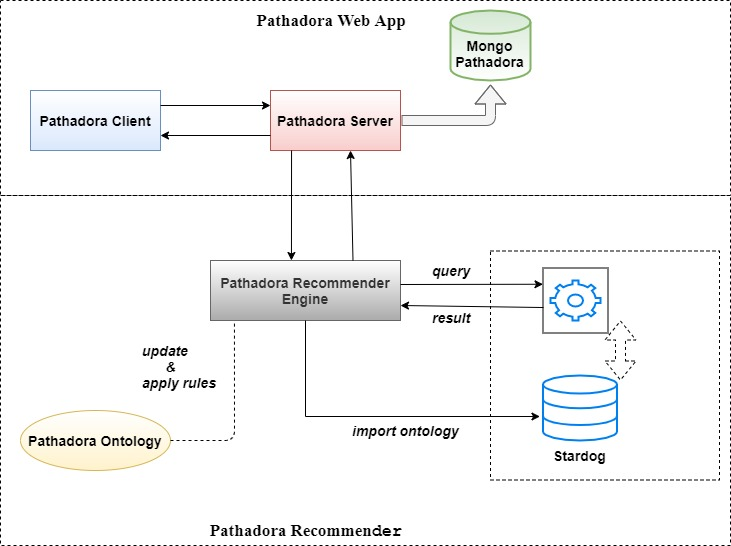
\includegraphics[scale=0.4]{res/pathadora-arch.jpg}
\caption{Architettura di Pathadora}
\label{fig:pathadora-arch}
\end{figure}

\begin{figure}[H]
\centering
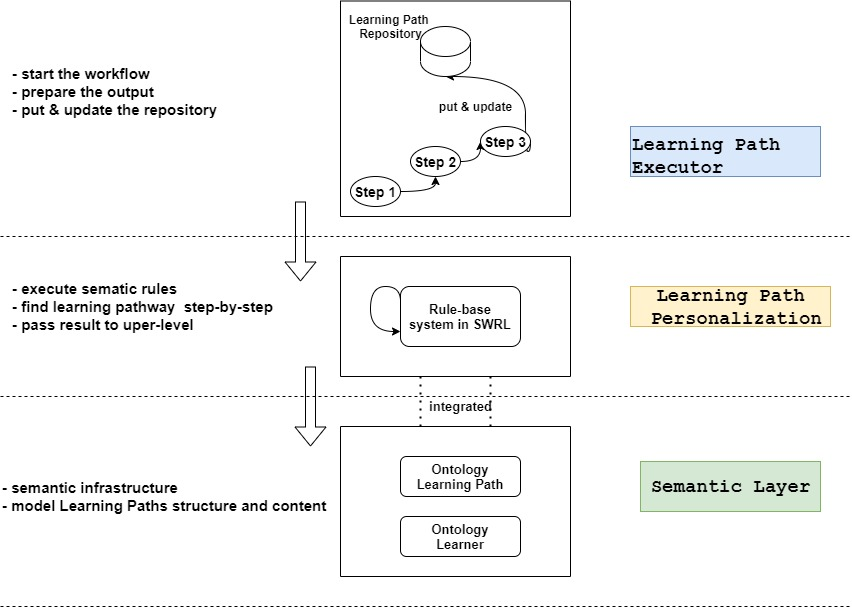
\includegraphics[scale=0.4]{res/diag-layers.jpg}
\caption{Workflow del sistema di raccomandazione}
\label{fig:diag-layers}
\end{figure}

\begin{figure}[H]
\centering
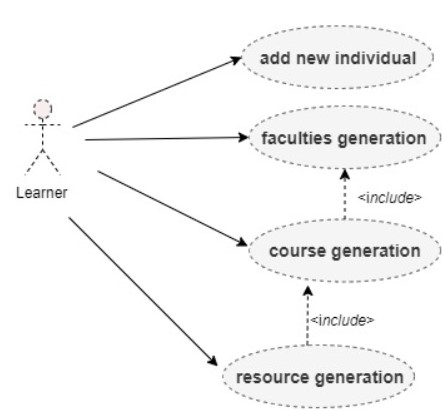
\includegraphics[scale=0.4]{res/pathadora-engine.jpg}
\caption{Casi d'uso sul Pathadora Recommender Engine}
\label{fig:pathadora-engine}
\end{figure}

\subsection{Richieste}
L'interfaccia web permette l'invio di richieste da sottomettere al Pathadora Engine attraverso appositi form.

\subsubsection{Inserimento}
La prima tipologia di richiesta da gestire è l’inserimento di nuove istanze nell'ontologia. In questa richiesta dovranno essere specificate tutte le informazioni che serviranno all’engine per aggiornare il knowledge graph. La richiesta potrebbe dichiarare relazioni tra elementi che non sono presenti e in tal caso, l’engine prima creerà questi elementi per poi definire la relazione tra
loro. Nel caso della richiesta di inserimento tutti gli elementi verranno aggiunti nell’ontologia, indipendentemente se esistono, se rispettano il formato giusto oppure se le relazioni sono semanticamente corrette.

Le informazioni inserite riguardano le lingue conosciute, i titoli di laurea corrente e futuro, le passioni per determinati settori, gli obiettivi dello studente e il possedimento di determinate disabilità con relativi livelli associati.

\subsubsection{Generazione di dipartimenti e facoltà}
A seguito della registrazione, lo studente può richiedere la generazione dei dipartimenti e delle facoltà suggerite, specificando il tipo di laurea (triennale, magistrale, dottorato) a cui fare riferimento. La generazione terrà conto delle informazioni dichiarate dallo studente durante la registrazione.

\begin{figure}[H]
\centering
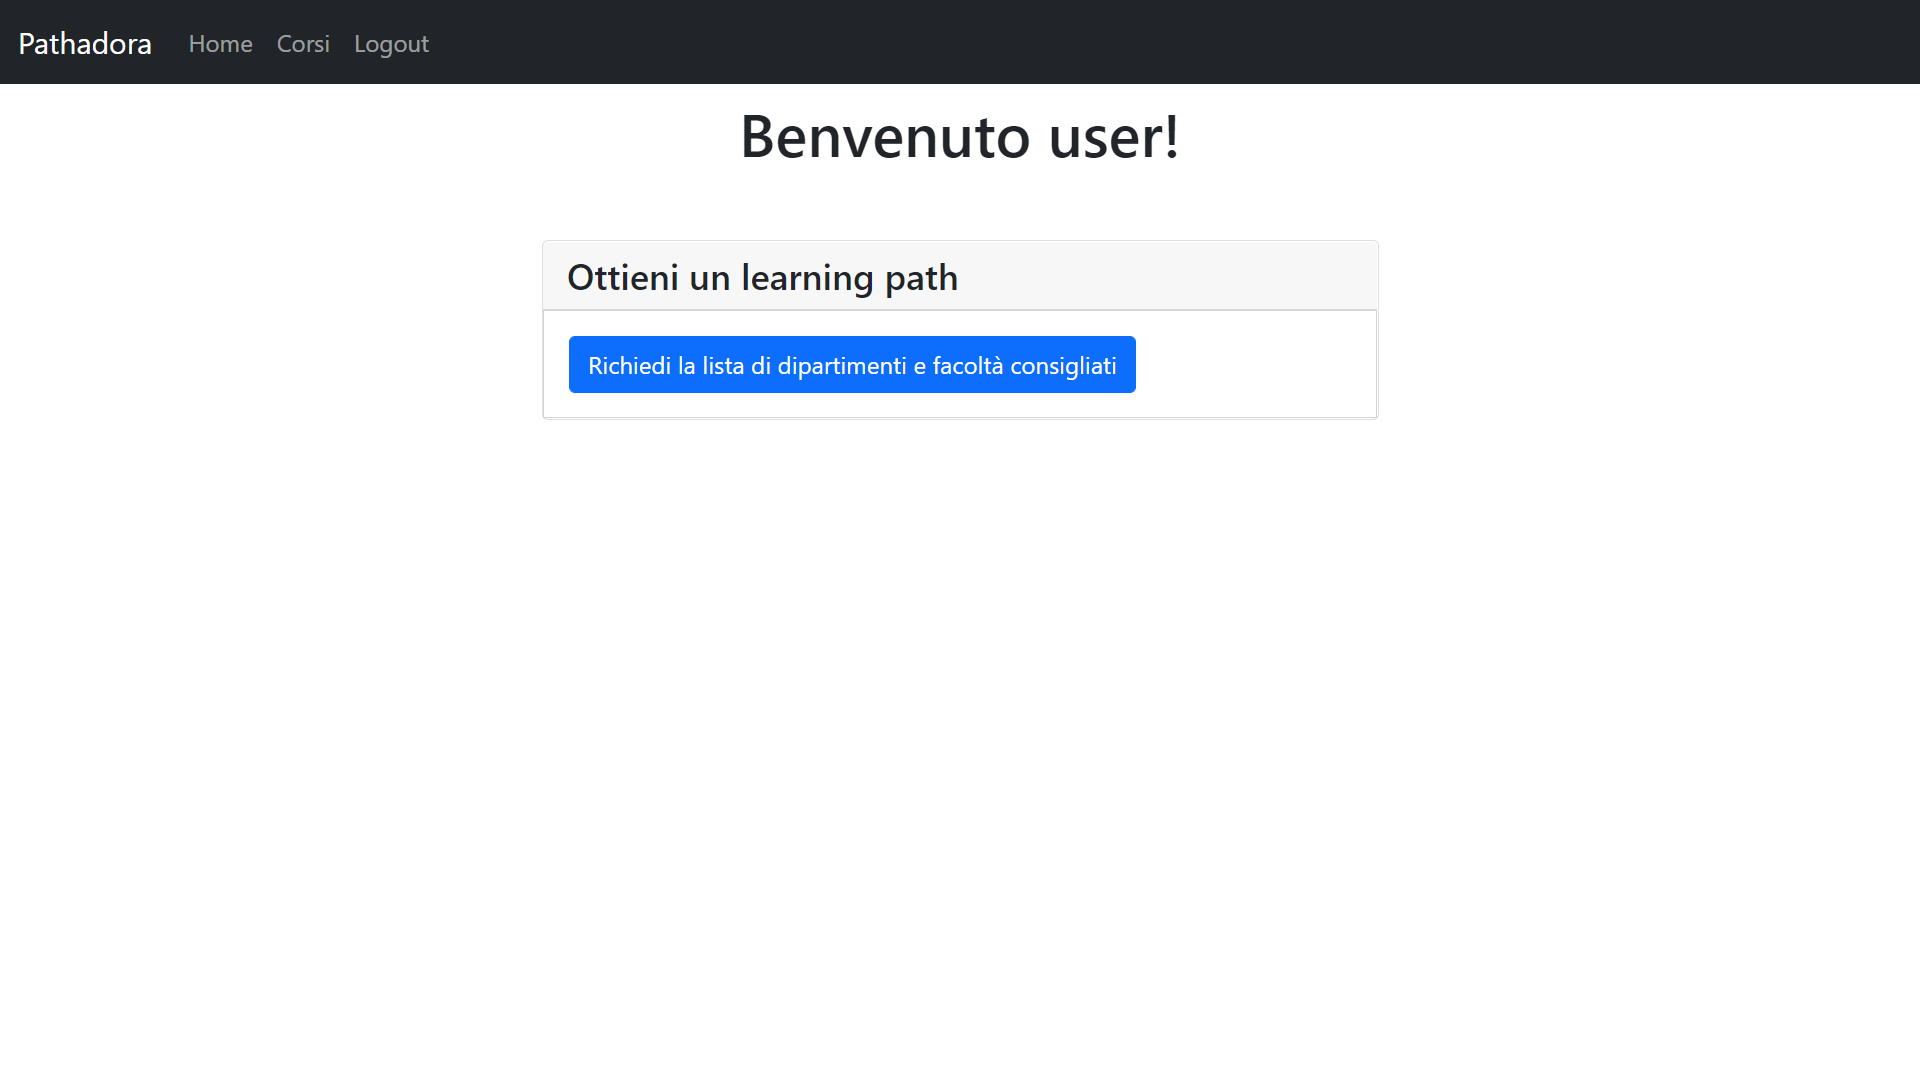
\includegraphics[scale=0.4]{res/faculties-generation.png}
\caption{Form di richiesta dipartimenti e facoltà suggeriti}
\label{fig:faculties-generation}
\end{figure}

\subsubsection{Generazione di corsi}
Una volta generate le facoltà, lo studente può richiedere la generare dei corsi suggeriti selezionando la facoltà e l'anno preferiti. 
Una volta ricevuto tale scelta, il sistema inizializzerà il knowledge graph e lo interrogherà parametrizzando la query con le informazioni dello studente.

\begin{figure}[H]
\centering
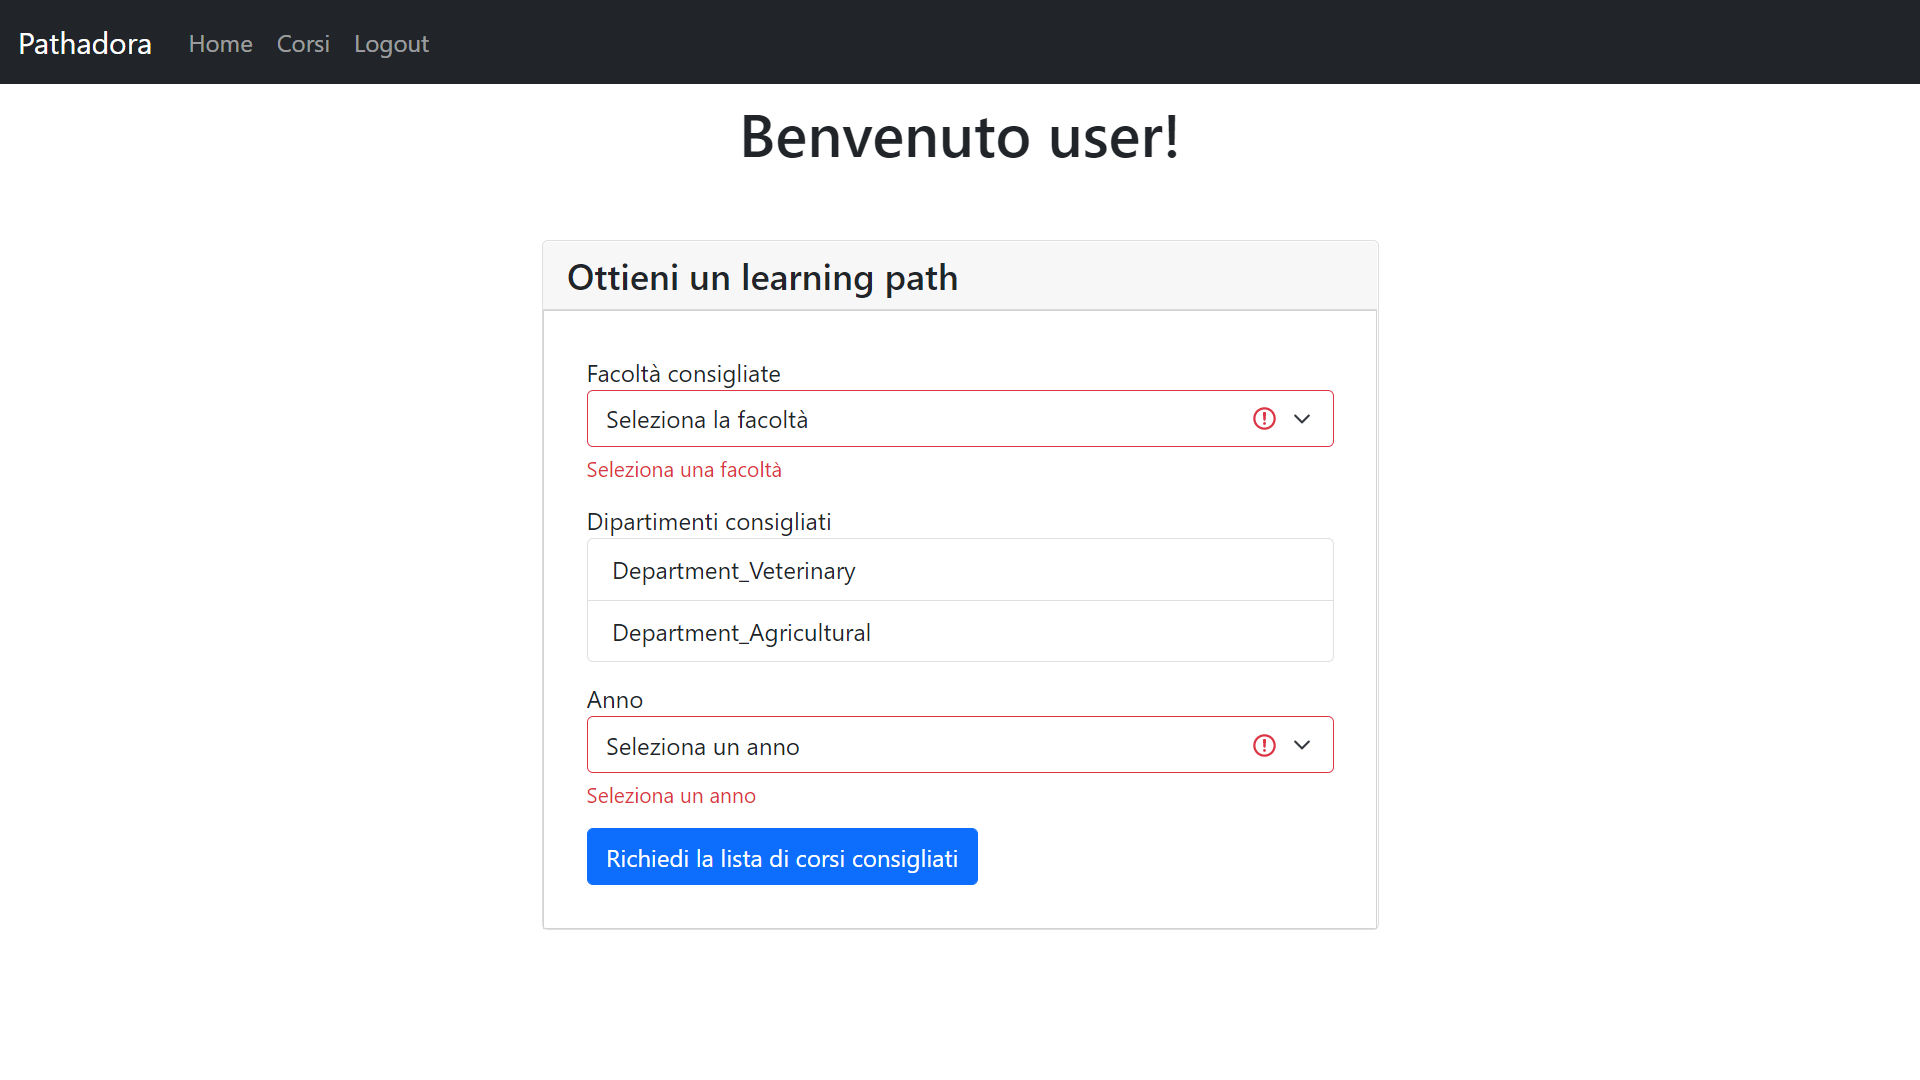
\includegraphics[scale=0.4]{res/courses-generation.png}
\caption{Form di richiesta corsi suggeriti}
\label{fig:courses-generation}
\end{figure}

\subsubsection{Generazione di risorse}
L'ultima richiesta da gestire consiste nella raccomandazione delle risorse relative a un corso specifico tra quelli suggeriti, risultati della richiesta precedente.
La raccomandazione terrà conto delle disabilità dello studente per determinare le risorse da raccomandare allo studente, a cui possono essere associate informazioni relative all'accessibilità come il grado di leggibilità del testo e la dimensione minima del font di un documento.

\begin{figure}[H]
\centering
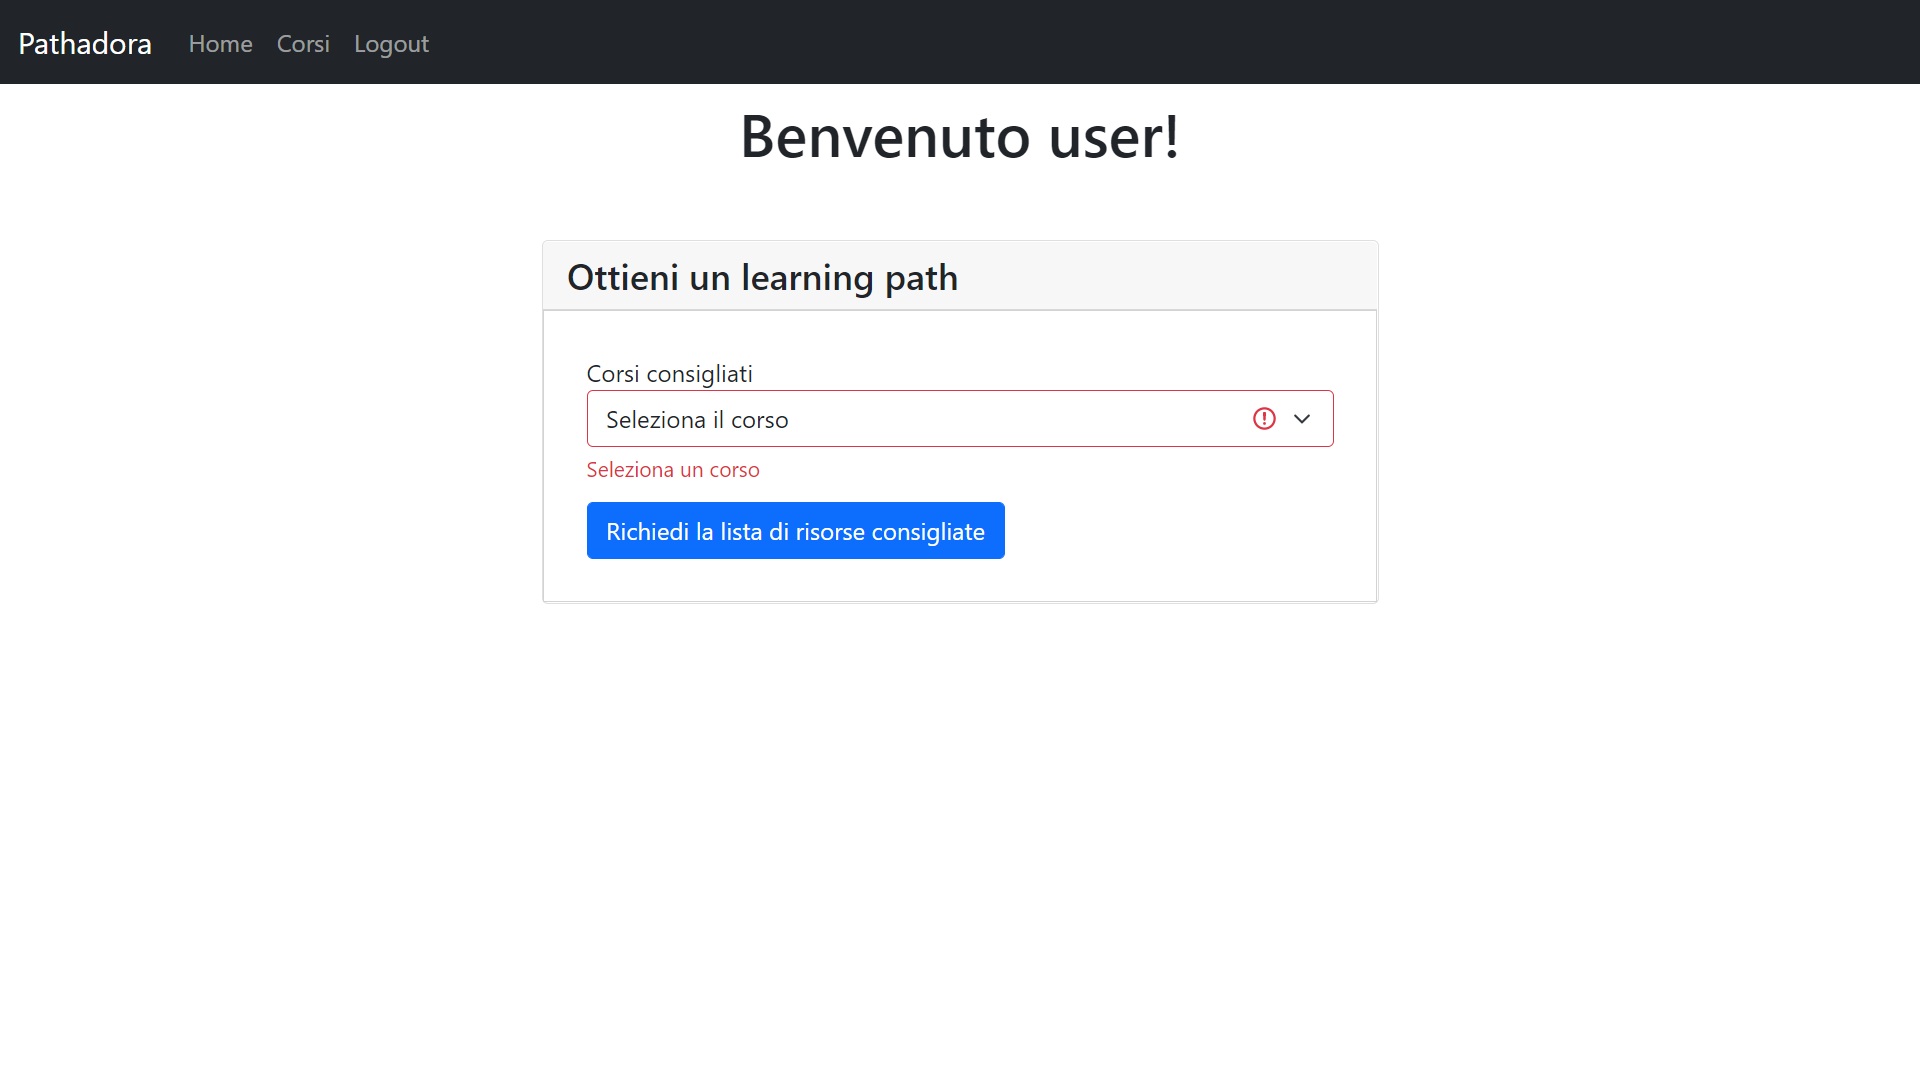
\includegraphics[scale=0.4]{res/resources-generation.png}
\caption{Form di richiesta risorse suggerite}
\label{fig:resources-generation}
\end{figure}

\begin{figure}[H]
\centering
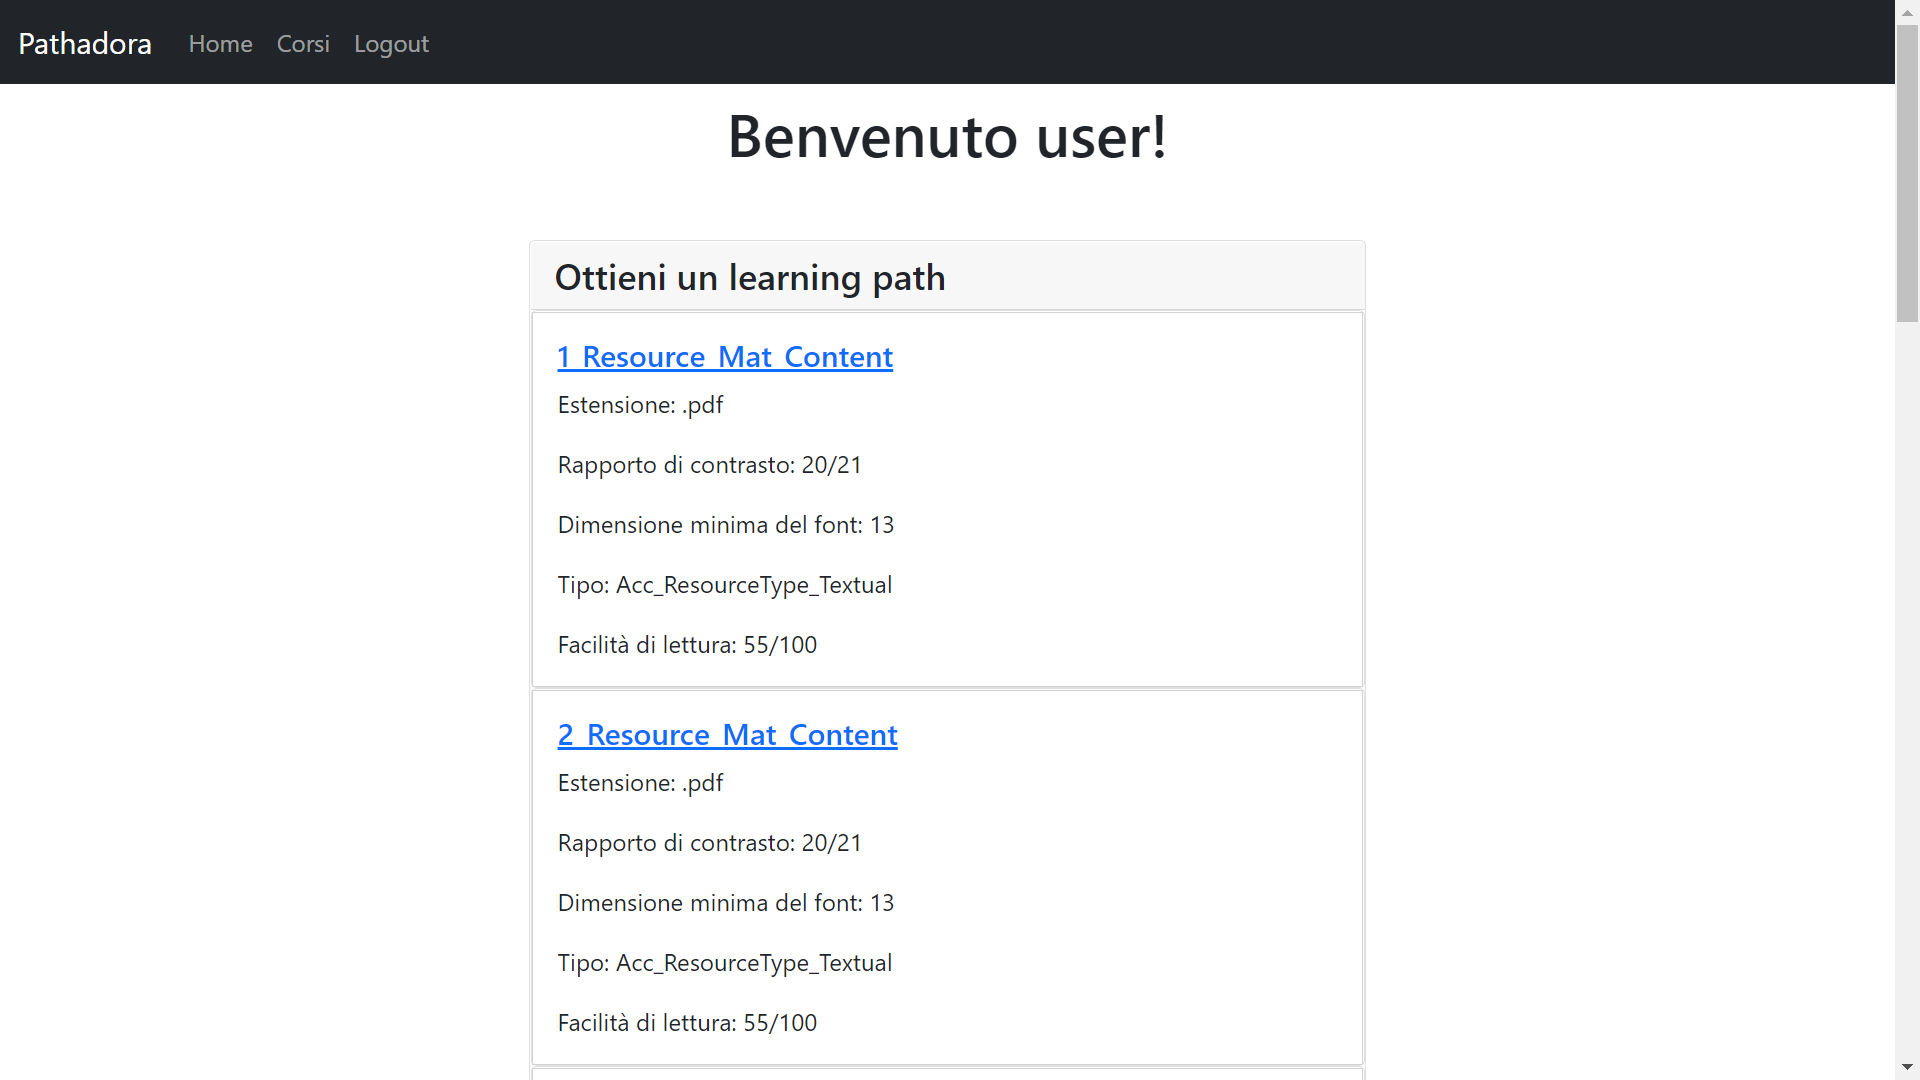
\includegraphics[scale=0.4]{res/path-result.png}
\caption{Risultato risorse suggerite}
\label{fig:resources-generation}
\end{figure}